\documentclass[10pt,a4paper]{report}
\usepackage{geometry}
\geometry{a4paper, left=30mm, right=20mm, top=30mm, bottom=20mm}
\setlength{\parindent}{4em}
\setlength{\parskip}{1em}
\renewcommand{\baselinestretch}{2.0}
\usepackage{indentfirst}

\usepackage[T1]{fontenc} 
\usepackage{multirow}
\usepackage{xcolor}
\newcommand{\beginsupplement}{%
        \setcounter{table}{0}
        \renewcommand{\thetable}{S\arabic{table}}%
        \setcounter{figure}{0}
        \renewcommand{\thefigure}{S\arabic{figure}}%
     }
     
\usepackage[font=small,labelfont=bf]{caption}
\usepackage{subcaption}%figure}
\usepackage{verbatim}
\usepackage{minted}
\usepackage{amsmath}
\usepackage{enumerate}
\usepackage{graphicx}
\usepackage{url}

\usepackage{titlesec}
\titleformat{\chapter}
  {\normalfont\Large\bfseries}
  {\thechapter.}
  {.5em}
  {\MakeUppercase}
  [\vspace{.5ex}{\titlerule[2pt]}]

%%%%%%%%%%%%%%%%%%%%%%%%%%%%%%%%%%%%%%%%%%%%%%%%%%%%%%%%%%%%%%%%%%%%%%%%%%%%%%%%%%%%%%%%%%%%%%%%%%%%%%%%%%%%%%%%%%%%%%%%%%%%%%%%%%%%%%%%%%%%%%%%%%%%%%%%%%%
\begin{document}

\begin{center}

  \vfill

  \textbf{\Huge{\textit{Themis} user guide}}

  \vfill

  \textbf{\Large{Version 1.0.0}}
  
  \vfill

\end{center}

\newpage

\begin{center}
  
  \vfill

  \noindent

  \textbf{\Large{\textit{Themis}: a Software to Assess Association Free Energies Via Direct Estimative of Partition Functions}}

  \vfill

  {Felippe Mariano Colombari}, {Kalil Bernardino}, {Weverson Rodrigues Gomes}, {Asdrubal Lozada Blanco} and
  {Andr\'e Farias de Moura} 

  \vfill

\end{center}

\newpage

\chapter{About}

  \textit{Themis} is a statistichal mechanics software designed to obtain the 
association thermodynamics of two structures (ions, molecules, crystals, 
nanoparticles, etc). It generates a configurational partition function by 
systematically sampling the phase space using discrete grids to perform 
translations and rotations of one structure around another. Interaction energy 
for each microstate can be obtained by one of the potentials implemented or 
by using external softwares.

  \textit{Themis} is a free software written in Fortran 2003 language, being 
available at \url{http://www.lqt.dq.ufscar.br/lqt/lqt_software-pt.html} under 
the GPLv3+ License. It runs under Linux environment with gfortran/gcc 5.4+ 
compilers. Since it was written in modules, new potential functions and analysis 
routines can be easily implemented.

\clearpage

\chapter{Obtaining a copy and compiling}

\chapter{Command line options}

  Themis usage is done via Linux command line as follows:

  \texttt{ themis [RUNTYPE] [GRID] }

  [RUNTYPE] options are:

  \texttt{---run} to start a new calculation.

  \texttt{---rerun} to calculated properties from interaction energies obtained previously. 
  In this case, an \texttt{energy.bin} file will be read if these energy values were obtained
  with Themis of an \texttt{energy.log} file will be read if these energy values were obtained
  externally. While ther former is useful in order to obtain thermodynamic properties using 
  a different temperature from a previous calculation, the latter is useful in order to obtain 
  thermodynamic properties using quantum chemistry interaction energies.

  [GRID] options are:

  \texttt{---shell <radius>} indicates that translation moves will be performed on a spherical 
  shell around the reference molecule (generated on the run). The real argument <radius> is the
  scaling factor for the radius (in Angstrom).

  \texttt{---user <file.xyz>} indicates that translation moves will be performed on an 
  user-defined grid read from <file.xyz>. It must be aligned with molecule 1 and can be generated 
  using the \texttt{sas\_grid} utility.

  This description can be seen using the \texttt{---help} flag.

\newpage

\chapter{Input files}

  \textbf{conf1.xyz}, \textbf{conf2.xyz} 
  
  Standard XYZ files containing the
coordinates of both structures. For the water dimer mentioned in the previous
sections, a dummy site (X) corresponding to water center of mass was used to
define the rotation axis of MOL1. \\~

\begin{center}
  \begin{minipage}{0.45\textwidth}
    \begin{minted}[fontsize=\scriptsize,gobble=2,baselinestretch=1.5,escapeinside=!!,frame=lines,framerule=1pt]{bash}

  themis@linux:~$ cat conf1.xyz 

    !4 
    *blank line*
    OW      0.00000      0.06682      0.00000
    HW     -0.76677     -0.53032      0.00000
    HW      0.76677     -0.53032      0.00000
    X       0.00000      0.00000      0.00000!

  themis@linux:~$ 

    \end{minted}
    \vskip0.5cm
  \end{minipage}%
%
  \hskip1.0cm
%
  \begin{minipage}{0.45\textwidth}
    \begin{minted}[fontsize=\scriptsize,gobble=2,baselinestretch=1.5,escapeinside=!!,frame=lines,framerule=1pt]{bash}

  themis@linux:~$ cat conf2.xyz 

    !4 
    *blank line*
    OW      0.00000      0.06682      0.00000
    HW     -0.76677     -0.53032      0.00000
    HW      0.76677     -0.53032      0.00000
    X       0.00000      0.00000      0.00000!

  themis@linux:~$

    \end{minted}
    \vskip0.5cm
  \end{minipage}%
\end{center}

%%%%%%%%%%%%%%%%%%%%%%%%%%%%%%%%%%%%%%%%%%%%%%%%%%%%%%%%%%%%%%%%%%%%%%%%%%%%%%%%%%%%%%%%%%%%%%%%%%%%%%%%%%%%%%%%%%%%%%%

\newpage
\textbf{INPUT} 

Plain text file containing detailed intructions prior to calculation. It must contain the following keywords:

\begin{center}
  \begin{minipage}{0.85\textwidth}
    \vskip0.25cm
    \begin{minted}[fontsize=\scriptsize,gobble=2,baselinestretch=1.5,escapeinside=!!,frame=lines,framerule=1pt]{bash}

  themis@linux:~$ cat INPUT 

    rot1_factor : !2          !              # integer
    translation_factor : !2   !              # integer
    rot2_factor :  !36        !              # integer
    rot2_range : !360.0       !              # real 
    temperature : !300.0      !              # real
    potential : !lj-coul      !              # character. valid strings are: none, lj-coul our bh-coul
    ref_mol1 : !1             !              # integer
    rot_ref_mol1 : !4         !              # integer
    ref_mol2 : !1             !              # integer
    rot_ref_mol2 : !2         !              # integer
    shortest_distance : !0.8  !              # real
    write_xtc : !no           !              # character. valid strings are: no, F, yes or T
    lowest_structures : !2    !              # integer
    write_frames : !none      !              # character. valid strings are: none, MOP or XYZ
    mopac_job :              !!              # character

  themis@linux:~$

    \end{minted}
  \end{minipage}%
\end{center}

\paragraph{rot1\_factor :} 

  Parameter ($p$) used to generate the spherical 
  grid used for reorientation moves. The number of points ($n$) obtained along 
  the sphere surface by dodecahedron tessellation (Figure~\ref{fig:spherical_grid}) 
  is given by $ n = 12 + 10 \times 3 \times ( p - 1 ) + 10 \times ( p - 2 ) \times ( p - 1 ) $.
  If one uses $p = 0$, the reorientation move will correspond to align molecule 2 along 
  Z-axis (1 reorientational move). 

\begin{figure}[!h]
  \begin{subfigure}[t]{0.18\textwidth}
    \center
    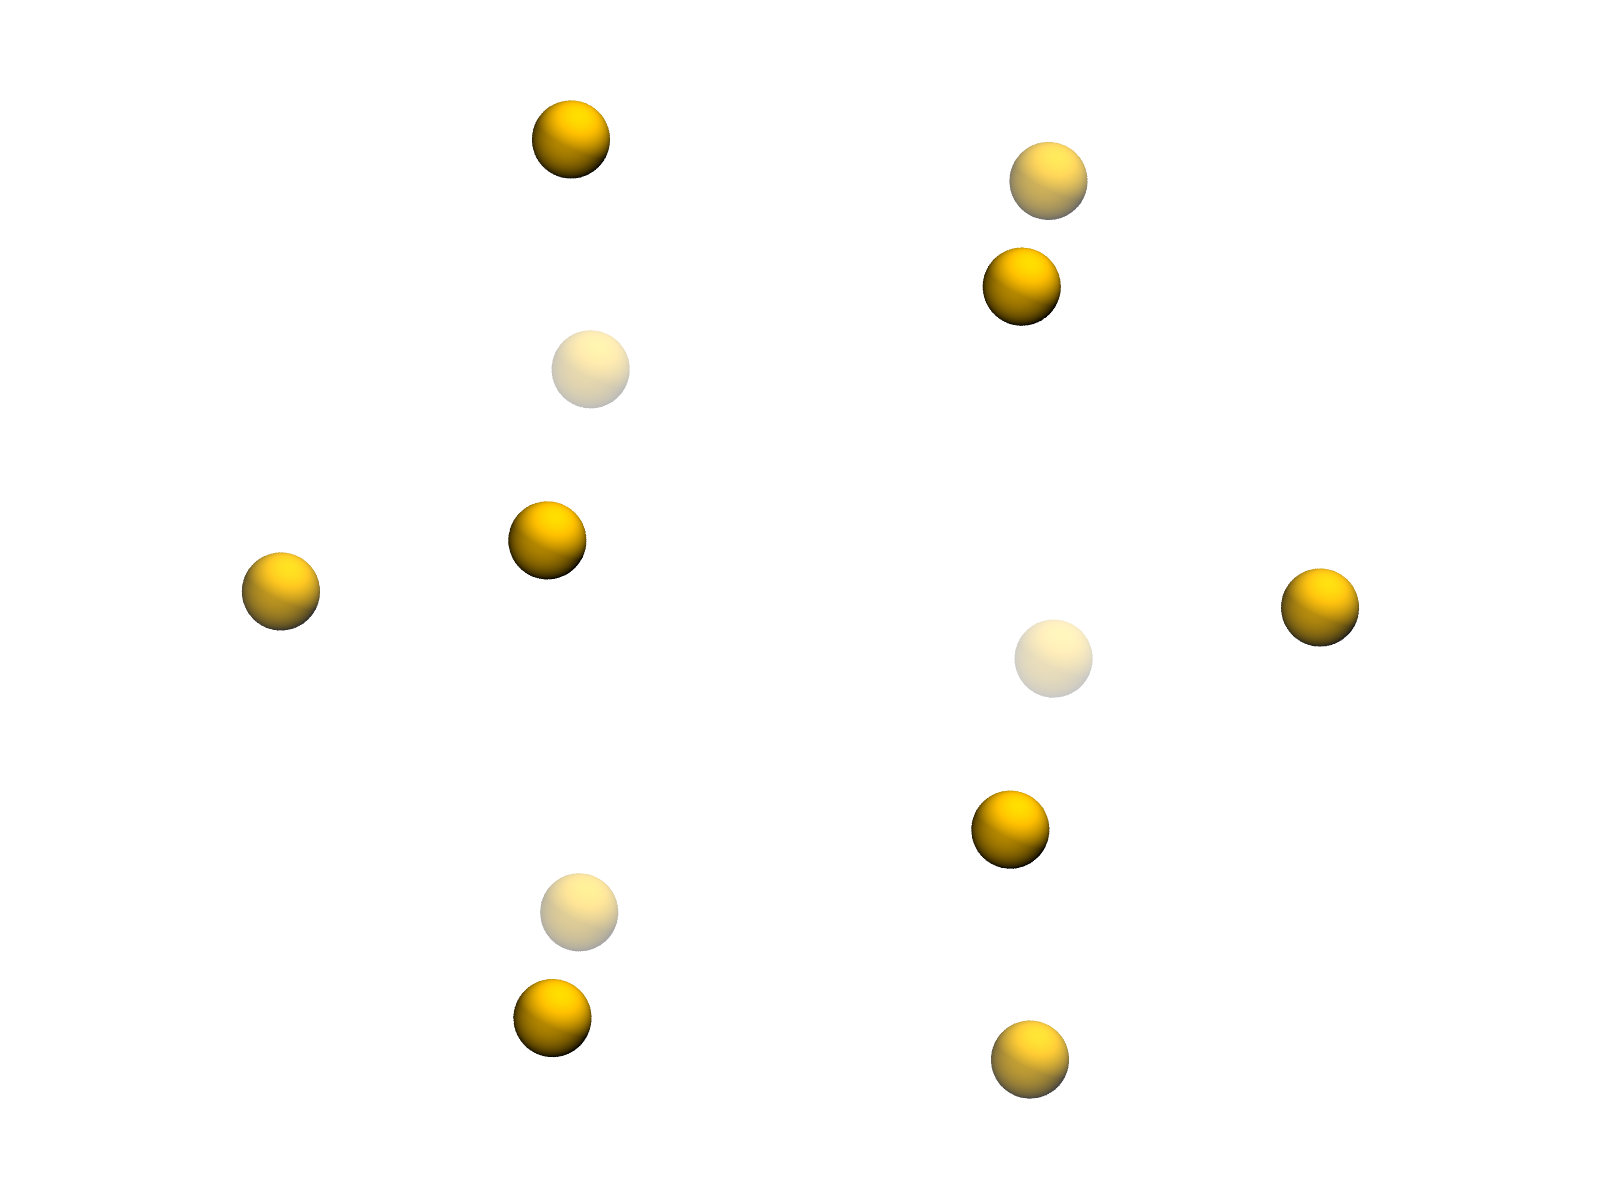
\includegraphics[width=\textwidth]{figures/grid_012.png}
    \footnotesize
    $p = 1$ \\
    $n = 12$
  \end{subfigure}
  \begin{subfigure}[t]{0.18\textwidth}
    \center
    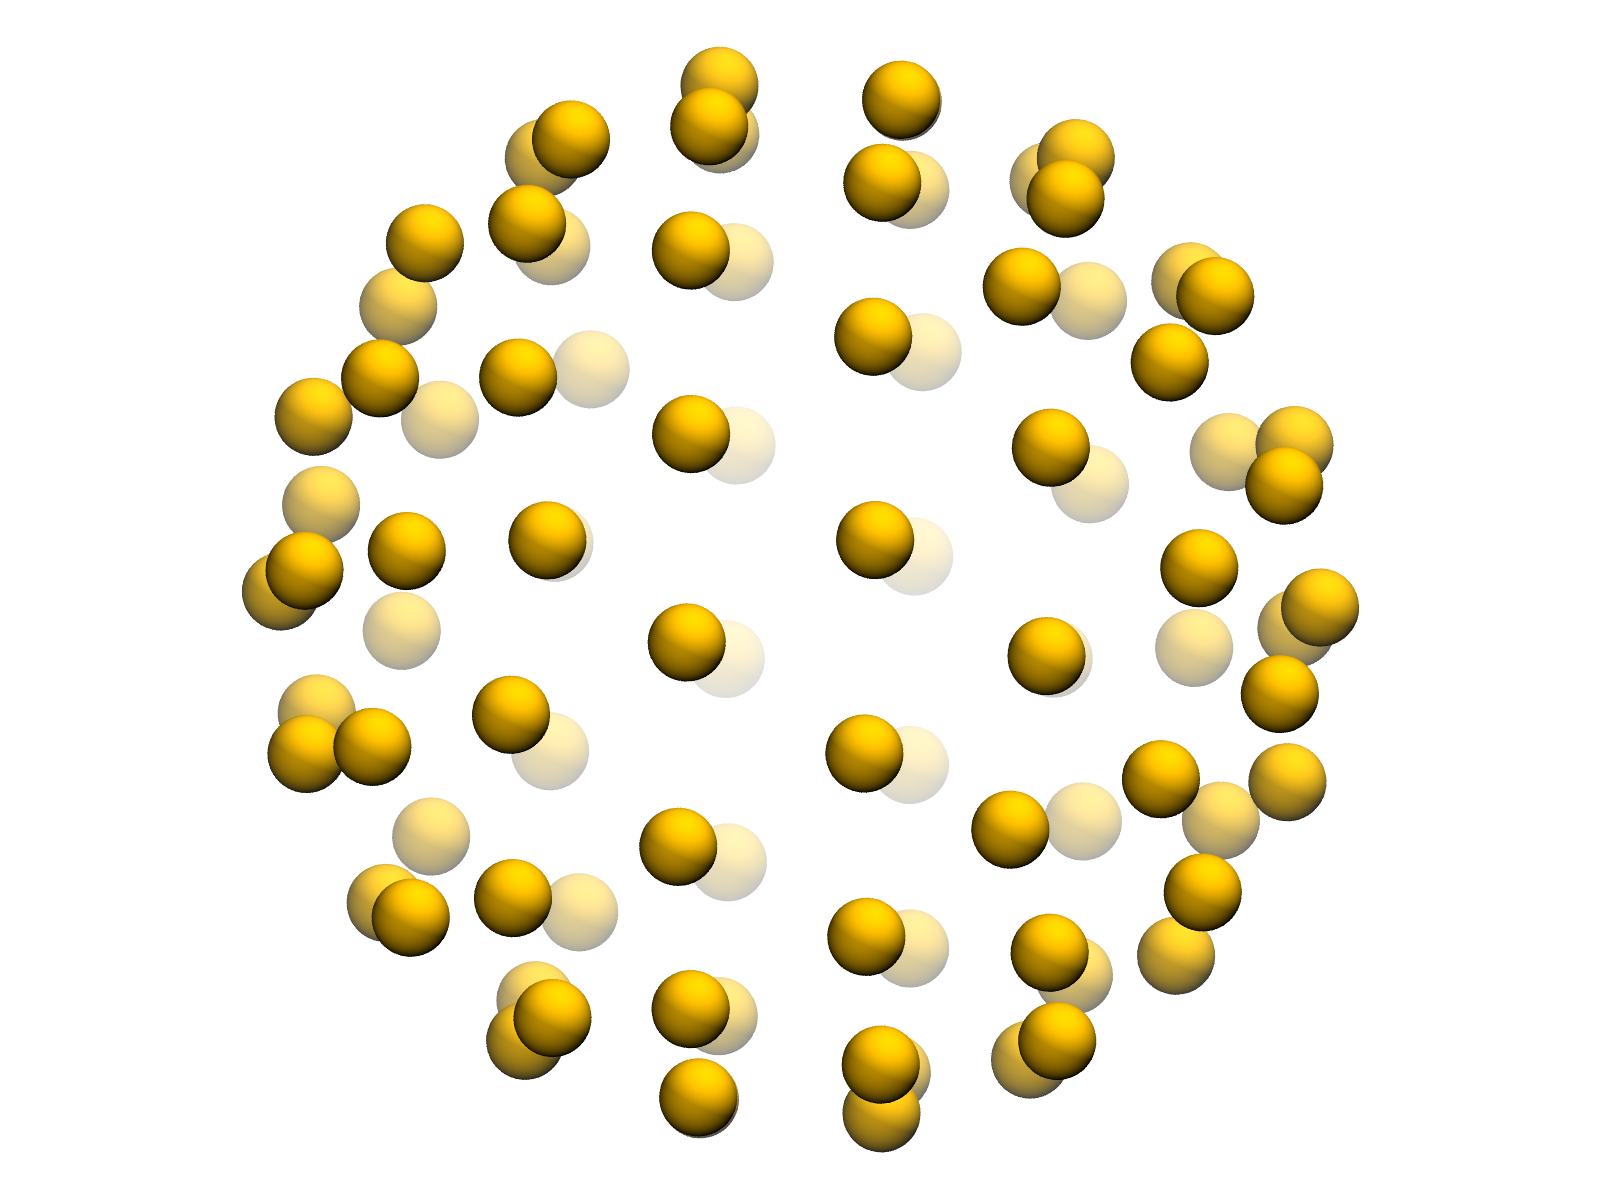
\includegraphics[width=\textwidth]{figures/grid_092.png} 
    \footnotesize
    $p = 3$ \\
    $n = 92$
  \end{subfigure}
  \begin{subfigure}[t]{0.18\textwidth}
    \center
    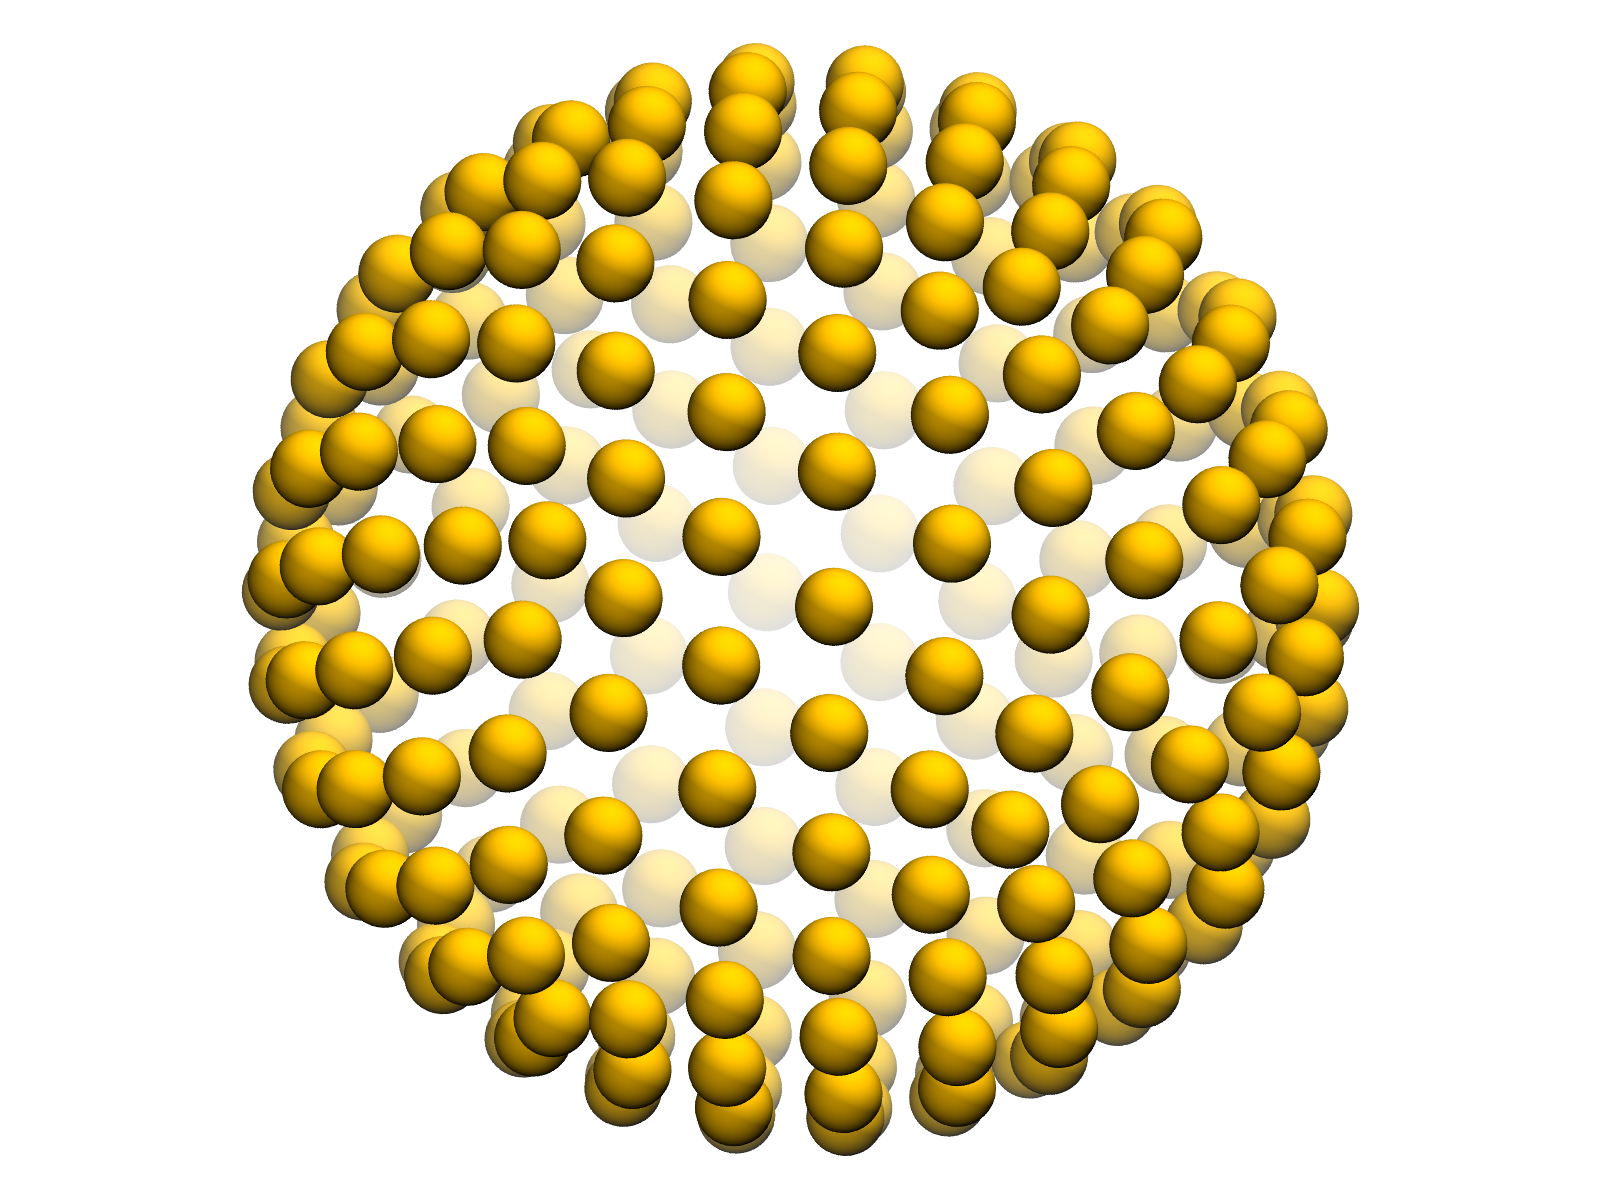
\includegraphics[width=\textwidth]{figures/grid_252.png} 
    \footnotesize
    $p = 5$ \\
    $n = 252$
  \end{subfigure}
  \begin{subfigure}[t]{0.18\textwidth}
    \center
    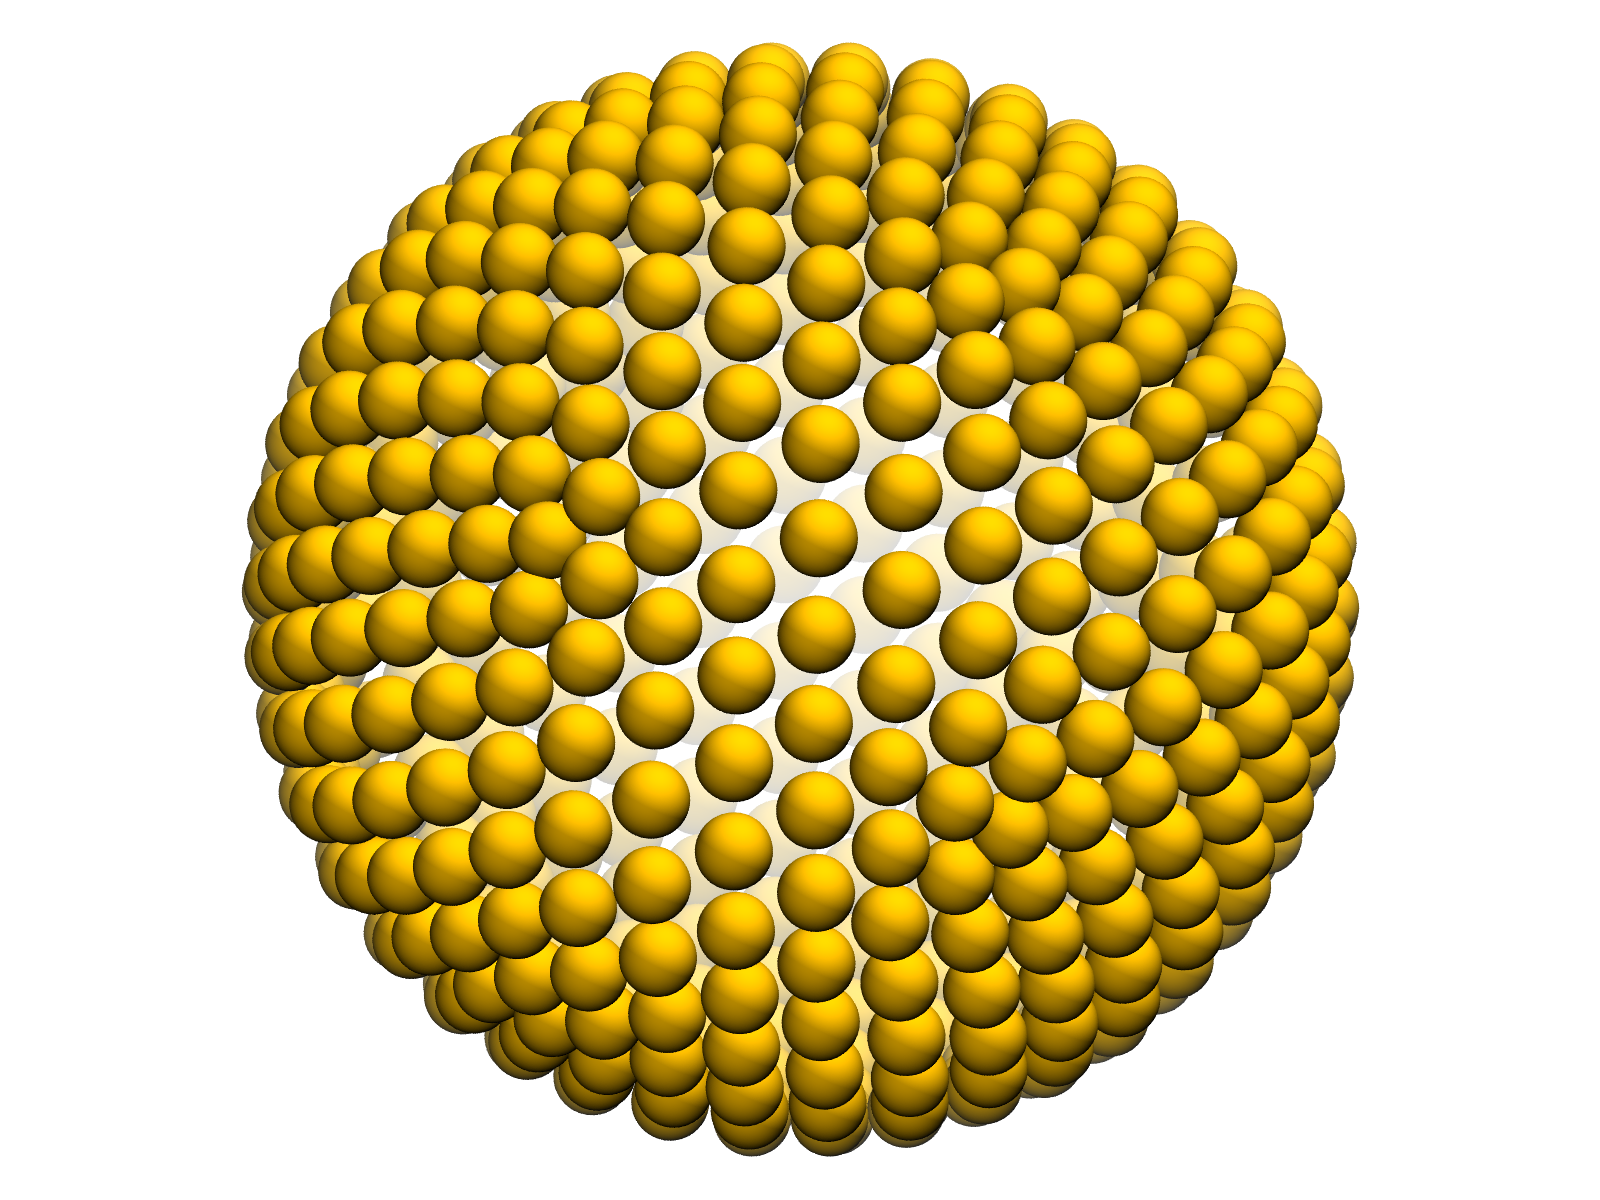
\includegraphics[width=\textwidth]{figures/grid_492.png} 
    \footnotesize
    $p = 7$ \\
    $n = 492$
  \end{subfigure}
  \begin{subfigure}[t]{0.18\textwidth}
    \center
    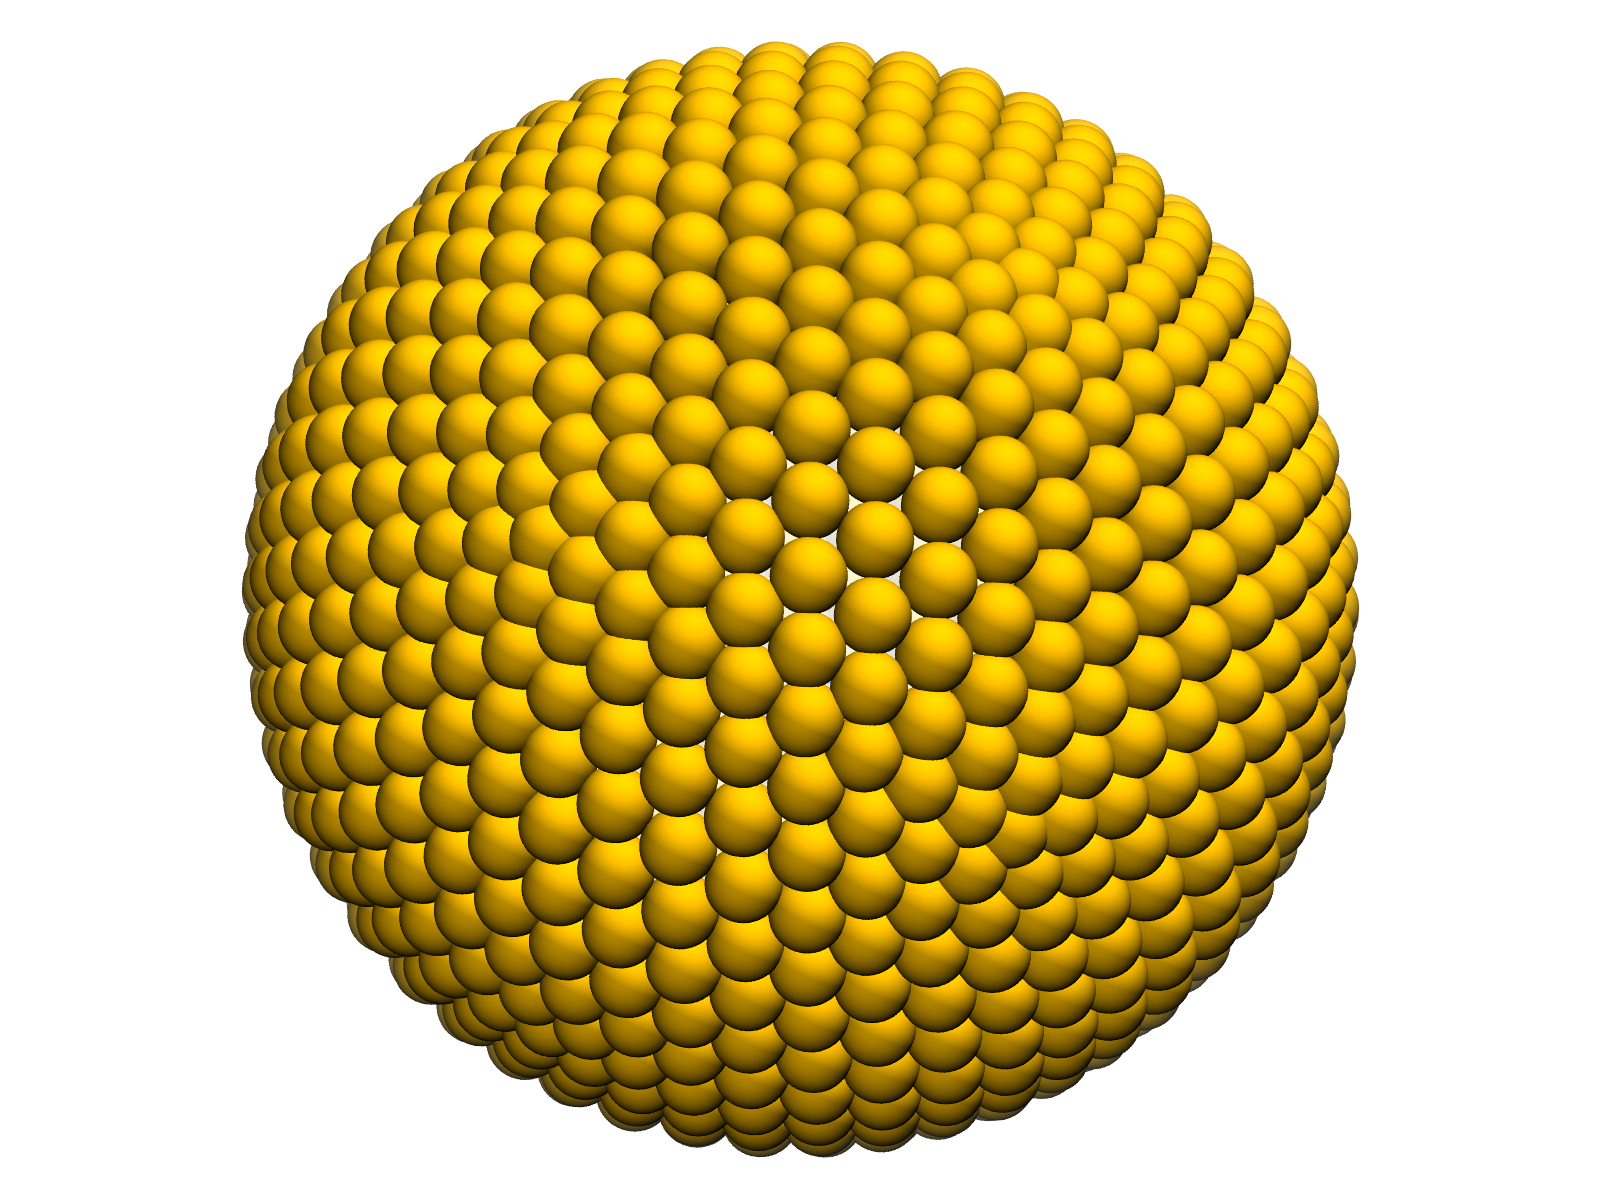
\includegraphics[width=\textwidth]{figures/grid_812.png} 
    \footnotesize
    $p = 9$ \\
    $n = 812$
  \end{subfigure}
  \caption{Spherical grids obtained by Tessellation.}
  \label{fig:spherical_grid}
\end{figure}


\paragraph{translation\_factor :} 

Same as \texttt{rot1\_factor} if a spherical translation shell is used.

\paragraph{rot2\_factor :} 

Corresponds to the number of rotation moves around the rotation axis. 
  
\paragraph{rot2\_range :} 

Corresponds to the maximum rotation angle (in degrees). 

\paragraph{temperature :} 

Absolute temperature (K) used to calculate all thermodynamic properties. 

\paragraph{potential :} 

Potential energy function selection. Options are ``none'', ``lj-coul'', ``bh-coul''. 

\paragraph{write\_frames :} 

Selects the format in which all valid frames will be written: ``XYZ'', ``MOP'' and ``none''. 
If ``MOP'' is selected, the optional character variable containing the first line of MOPAC 
input (\textbf{mopac\_job}) is read. 

\paragraph{ref\_mol1 :} 

Site of molecule 1 used for centering, according to \textbf{conf1.xyz} file. 

\paragraph{rot\_ref\_mol1 :} 

Site of molecule 1 that will build its rotation vector, according to \textbf{conf1.xyz} file. 

\paragraph{ref\_mol2 :} 

Site of molecule 2 used for centering, according to \textbf{conf2.xyz} file. 

\paragraph{rot\_ref\_mol2 :} 

Site of molecule 2 that will build its rotation vector, according to \textbf{conf2.xyz} file. 

\paragraph{shortest\_distance :} 

Corresponds to the lowest intermolecular distance to consider the configuration as a valid one. 
Below such value (in Angstrom), molecular contacts are considered strongly repulsive and an 
interaction energy value of $10^{10}$ kJ/mol is attributed  to such configuration. This is useful 
to avoid spending time calculating energies for unphisical configurations since the energy loop 
is skipped.

\paragraph{write\_xtc :} 

Flag to enable the writting of all configurations to a XTC file. WARNING: very large files can 
be generated ;) 
  
\paragraph{lowest\_structures :} 

Selects the number of lowest energy/highest probability structures to write after the run. 
  
\paragraph{mopac\_job :} 

String containing the header for mopac calculations. Enabled when ``write\_frames : MOP'' is selected.

%%%%%%%%%%%%%%%%%%%%%%%%%%%%%%%%%%%%%%%%%%%%%%%%%%%%%%%%%%%%%%%%%%%%%%%%%%%%%%%%%%%%%%%%%%%%%%%%%%%%%%%%%%%%%%%%%%%%%%%

  \textbf{parameters1}, \textbf{parameters2} 

  Plain text files containing 
potential parameters used for energy calculations. Those files are read differently 
according to the potential used. For Lennard-Jones + Coulomb interaction potential 
(invoked by \texttt{potential:lj-coul}), one should provide $q_{i}$, $\sigma_{i}$ 
and $\epsilon_{i}$ parameters, according to Equation~\ref{eqn:ljc}

\begin{equation}
  \label{eqn:ljc}
  U_{\textrm{ljc}} =  
  \sum\limits_{i} \sum\limits_{j<i}4\epsilon_{ij}\bigg[\bigg(\frac{\sigma_{ij}}{r_{ij}}\bigg)^{\!\!12}
  -\bigg(\frac{\sigma_{ij}}{r_{ij}}\bigg)^{\!\!6}\bigg]
	+\frac{1}{4\pi\varepsilon_{0}}\sum\limits_{i} \sum\limits_{j<i}\frac{q_{i}q_{j}}{r_{ij}}
\end{equation}

where $\epsilon_{ij} = ( \epsilon_{i} \cdot \epsilon_{j})^\frac{1}{2}$ and
$\sigma_{ij} = ( \sigma_{i} \cdot \sigma_{j})^\frac{1}{2}$. TIP3P parameter files for 
water are read as follows:

\begin{center}
  \begin{minipage}{0.45\textwidth}
    \vskip0.25cm
    \begin{minted}[fontsize=\scriptsize,gobble=2,baselinestretch=1.5,escapeinside=!!,frame=lines,framerule=1pt]{bash}

  themis@linux:~$ cat parameters1

    !#   q          sig (A)     eps (kJ/mol)
    OW  -0.834     3.15061     0.636386
    HW  +0.417     0.00000     0.000000	 
    HW  +0.417     0.00000     0.000000	 
    X    0.000     0.00000     0.000000!

  themis@linux:~$

    \end{minted}
  \end{minipage}%
%
  \hskip0.5cm
%
  \begin{minipage}{0.45\textwidth}
    \vskip0.25cm
    \begin{minted}[fontsize=\scriptsize,gobble=2,baselinestretch=1.5,escapeinside=!!,frame=lines,framerule=1pt]{bash}

  themis@linux:~$ cat parameters2

    !#   q          sig (A)     eps (kJ/mol)
    OW  -0.834     3.15061     0.636386
    HW  +0.417     0.00000     0.000000	 
    HW  +0.417     0.00000     0.000000	 
    X    0.000     0.00000     0.000000!

  themis@linux:~$

    \end{minted}
  \end{minipage}%
\end{center}

  For Buckingham + Coulomb interaction potential, according to
Matsui~\cite{matsui}, one should invoke \texttt{potential:bh-coul} 
and provide $A_{i}$, $B_{i}$ and $C_{i}$ parameters according to (eq.~\ref{eqn:bhc})

\begin{equation}
  \label{eqn:bhc}
  U_{\textrm{bhc}} =  
  \sum\limits_{i}
  \sum\limits_{j<i}\bigg\{\bigg(\frac{-C_{i}C_{j}}{r_{ij}^{6}}\bigg)
  + f(B_{i}+B_{j})
\exp\bigg[\bigg(\frac{A_{i}+A_{j}-r_{ij}}{B_{i}+B_{j}}\bigg)\bigg]\bigg\}
	+\frac{1}{4\pi\epsilon_{0}}\sum\limits_{i} \sum\limits_{j<i}\frac{q_{i}q_{j}}{r_{ij}}
\end{equation}

where the quantity $f$ corresponds to a standard force of 4.184 kJ/mol/\AA. Parameters 
for a TiO$_{2}$ unit must be provided as follows:

\begin{center}
  \begin{minipage}{0.45\textwidth}
    \vskip0.25cm
    \begin{minted}[fontsize=\scriptsize,gobble=2,baselinestretch=1.5,escapeinside=!!,frame=lines,framerule=1pt]{bash}

  themis@linux:~$ cat parameters1

   !#   q          A(A)      B (A)     C(A**3 kJ/mol)
   Ti   2.1960    1.18230   0.07700   22.5000
   O   -1.0980    1.63390   0.11700   54.0000
   O   -1.0980    1.63390   0.11700   54.0000
   X    0.0000    0.00000   0.00000   0.00000!

  themis@linux:~$

    \end{minted}
  \end{minipage}%
%
  \hskip0.75cm
%
  \begin{minipage}{0.45\textwidth}
    \vskip0.25cm
    \begin{minted}[fontsize=\scriptsize,gobble=2,baselinestretch=1.5,escapeinside=!!,frame=lines,framerule=1pt]{bash}

  themis@linux:~$ cat parameters2

   !#   q         A(A)      B (A)     C(A**3 kJ/mol)
   Ti  2.1960    1.18230   0.07700   22.5000
   O  -1.0980    1.63390   0.11700   54.0000
   O  -1.0980    1.63390   0.11700   54.0000
   X   0.0000    0.00000   0.00000   0.00000!

  themis@linux:~$

    \end{minted}
  \end{minipage}%
\end{center}

  \textbf{NOTE:} It is important to highlight that atoms described in both \texttt{parameters1}
and \texttt{parameters2} files must be in the same order as they appear in both 
\texttt{conf1.xyz} and \texttt{conf2.xyz} files. Parameters file must contain a 
header followed by one line for each atom descrived in structure files.

%%%%%%%%%%%%%%%%%%%%%%%%%%%%%%%%%%%%%%%%%%%%%%%%%%%%%%%%%%%%%%%%%%%%%%%%%%%%%%%%%%%%%%%%%%%%%%%%%%%%%%%%%%%%%%%%%%%%%%%

\newpage

\chapter{Output files}

\textbf{energy.bin}

  Binary file containing interaction energy values for all microstates. Since
  all entries are written in the right loop sequence, they can be read using the
  \texttt{rerun} feature. \\~

\textbf{energy-sort.log}
  
  Contains interaction energy values and probabilities for the N most probable
  structures. By running Themis with the input files presented below, and
  considering a spherical grid with radius = 2.8 \AA, one obtains \\~

\begin{center}
  \begin{minipage}{0.75\textwidth}
    \vskip0.25cm
    \begin{minted}[fontsize=\scriptsize,gobble=2,baselinestretch=1.5,escapeinside=!!,frame=lines,framerule=1pt]{bash}

  themis@linux:~$ cat energy-sort.log

  #int_energy(r2,r1,t) r2      r1       t        prob.     sum prob.
    !-2.83500E+001       1      10       3     6.704E-004  6.704E-004
    -2.83500E+001       1       4       9     6.704E-004  1.341E-003
    -2.83453E+001       2       4       9     6.692E-004  2.010E-003
    -2.83453E+001       2      10       3     6.692E-004  2.679E-003
    -2.83453E+001     120       4       9     6.692E-004  3.348E-003
    -2.83453E+001     120      10       3     6.692E-004  4.017E-003
    -2.83312E+001       3      10       3     6.654E-004  4.683E-003
    -2.83312E+001     119      10       3     6.654E-004  5.348E-003
    -2.83312E+001       3       4       9     6.654E-004  6.014E-003
    -2.83312E+001     119       4       9     6.654E-004  6.679E-003
    -2.83078E+001     118      10       3     6.592E-004  7.338E-003
    -2.83078E+001     118       4       9     6.592E-004  7.997E-003
    -2.83078E+001       4      10       3     6.592E-004  8.657E-003
    -2.83078E+001       4       4       9     6.592E-004  9.316E-003
    -2.82751E+001     117       4       9     6.506E-004  9.966E-003
    -2.82751E+001     117      10       3     6.506E-004  1.062E-002
    -2.82751E+001       5      10       3     6.506E-004  1.127E-002
    -2.82751E+001       5       4       9     6.506E-004  1.192E-002
    -2.82333E+001     116      10       3     6.398E-004  1.256E-002
    -2.82333E+001       6      10       3     6.398E-004  1.320E-002!

  themis@linux:~$ 

    \end{minted}
  \end{minipage}%
\end{center}

\textbf{output.log}

  Contains thermodynamic data for all translation grid points, and also for the
  overall ensemble. Written in an extended XYZ format containing extra field values 
  for each grid point (probability, free energy, energy and entropic penalty). \\~


\begin{center}
  \begin{minipage}{0.90\textwidth}
    \vskip0.25cm
    \begin{minted}[fontsize=\scriptsize,gobble=2,baselinestretch=1.5,escapeinside=!!,frame=lines,framerule=1pt]{bash}

  themis@linux:~$ cat output.log

           42
   #      X (A)     Y (A)     Z (A)  point           PROB      A (kJ/mol)    -TS (kJ/mol)      E (kJ/mol)
   !X    2.38182   1.47205   0.00000      1   2.98845E-003   -1.08134E+001    6.75915E+000   -1.75725E+001
   X    2.38182  -1.47205   0.00000      2   2.98845E-003   -1.08134E+001    6.75915E+000   -1.75725E+001
   X    1.47205   0.00000   2.38182      3   5.85172E-002   -1.82330E+001    6.84167E+000   -2.50746E+001
   X    1.47205   0.00000  -2.38182      4   1.34004E-003   -8.81280E+000    4.19575E+000   -1.30086E+001
   X    0.00000   2.38182   1.47205      5   1.00969E-002   -1.38502E+001    6.78551E+000   -2.06357E+001
   X    0.00000   2.38182  -1.47205      6   1.74725E-001   -2.09615E+001    4.32032E+000   -2.52818E+001
   X    0.00000  -2.38182   1.47205      7   1.00969E-002   -1.38502E+001    6.78551E+000   -2.06357E+001
   X    0.00000  -2.38182  -1.47205      8   1.74725E-001   -2.09615E+001    4.32032E+000   -2.52818E+001
   ...
   X   -2.26525   0.86525  -1.40000     40   9.83462E-004   -8.04111E+000    5.57165E+000   -1.36128E+001
   X   -2.26525  -0.86525  -1.40000     41   9.83462E-004   -8.04111E+000    5.57165E+000   -1.36128E+001
   X   -2.80000   0.00000   0.00000     42   2.97201E-003   -1.07996E+001    6.97190E+000   -1.77715E+001
   -------------------------------------------------------------------------------------------------------
   TOTAL OVER TRANSLATIONAL GRID             1.00000E+000   -1.59900E+001    7.67496E+000   -2.36649E+001!

  themis@linux:~$ 

    \end{minted}
  \end{minipage}%
\end{center}

\textbf{output-sort.log}

  Same as \texttt{output.log} but ordered from most probable point to the least 
  probable point. \\~ 

\begin{center}
  \begin{minipage}{0.90\textwidth}
    \begin{minted}[fontsize=\scriptsize,gobble=2,baselinestretch=1.5,escapeinside=!!,frame=lines,framerule=1pt]{bash}

  themis@linux:~$ cat output-sort.log

          42
   #      X (A)     Y (A)     Z (A)  point           PROB      A (kJ/mol)    -TS (kJ/mol)      E (kJ/mol)
   !X    0.00000  -2.38182  -1.47205      8   1.74725E-001   -2.09615E+001    4.32032E+000   -2.52818E+001
   X    0.00000   2.38182  -1.47205      6   1.74725E-001   -2.09615E+001    4.32032E+000   -2.52818E+001
   X    0.00000   0.00000   2.80000     24   8.68520E-002   -1.92179E+001    6.43659E+000   -2.56545E+001
   X    1.47205   0.00000   2.38182      3   5.85172E-002   -1.82330E+001    6.84167E+000   -2.50746E+001
   X   -1.47205   0.00000   2.38182      9   5.85172E-002   -1.82330E+001    6.84167E+000   -2.50746E+001
   X    0.86525   1.40000   2.26525     22   4.04675E-002   -1.73130E+001    7.12969E+000   -2.44427E+001
   X   -0.86525   1.40000   2.26525     29   4.04675E-002   -1.73130E+001    7.12969E+000   -2.44427E+001
   X    0.86525  -1.40000   2.26525     23   4.04675E-002   -1.73130E+001    7.12969E+000   -2.44427E+001
   ...
   X   -2.26525   0.86525  -1.40000     40   9.83462E-004   -8.04111E+000    5.57165E+000   -1.36128E+001
   X    2.26525  -0.86525  -1.40000     19   9.83462E-004   -8.04111E+000    5.57165E+000   -1.36128E+001
   X   -2.26525  -0.86525  -1.40000     41   9.83462E-004   -8.04111E+000    5.57165E+000   -1.36128E+001
   -------------------------------------------------------------------------------------------------------
   TOTAL OVER TRANSLATIONAL GRID             1.00000E+000   -1.59900E+001    7.67496E+000   -2.36649E+001!

  themis@linux:~$ 

    \end{minted}
    \vskip0.25cm
  \end{minipage}%
\end{center}

\textbf{surf\_free-energy.vmd, surf\_energy.vmd, surf\_entropic-penalty.vmd} 

  Contains a VMD script for reading the thermodynamic data along the translation
  grid from file \texttt{output.log}. \\~

\textbf{lowest\_0001.xyz}
  
  XYZ coordinates for the most probable structure from the whole ensemble. The
  number of lowest structure files is defined by the user in the \texttt{INPUT}
  file. \\~

\begin{center}
  \begin{minipage}{0.5\textwidth}
    \begin{minted}[fontsize=\scriptsize,gobble=2,baselinestretch=1.5,escapeinside=!!,frame=lines,framerule=1pt]{bash}

  themis@linux:~$ cat lowest_0001.xyz

    !         8
    Energy =  -2.8350000E+01
    O       0.0000     0.0000     0.0000
    H      -0.0000    -0.7668    -0.5971
    H      -0.0000     0.7668    -0.5971
    X      -0.0000    -0.0000    -0.0668
    O       1.4720     0.0000     2.3818
    H       0.9611     0.0000     1.5551
    H       0.7957     0.0000     3.0797
    X       1.4056     0.0000     2.3746!

  themis@linux:~$ 

    \end{minted}
    \vskip0.25cm
  \end{minipage}%
\end{center}


\textbf{grid\_log.log}

  File containing informations of each translation grid point: point number,
  number of rejected structures (due to atomic clashes), spent time. \\~

\begin{center}
  \begin{minipage}{0.40\textwidth}
    \begin{minted}[fontsize=\scriptsize,gobble=2,baselinestretch=1.5,escapeinside=!!,frame=lines,framerule=1pt]{bash}

  themis@linux:~$ cat grid_log.log

   !t point   rejected structures   time (s)
         1         0 of    5040      0.020
         2         0 of    5040      0.012
         3         0 of    5040      0.012
         4         0 of    5040      0.013
       ...
        38         0 of    5040      0.024
        39         0 of    5040      0.013
        40         0 of    5040      0.013
        41         0 of    5040      0.012
        42         0 of    5040      0.014!

  themis@linux:~$ 

    \end{minted}
    \vskip0.25cm
  \end{minipage}%
\end{center}

\textbf{full\_ensemble.xtc}

  XTC trajectory file containing the whole ensemble. Written if INPUT option
  \texttt{write\_xtc} is enabled. \\~

\textbf{point\_0001\_0001\_0001.xyz}

  XYZ file containing the structure of the microstate t = 1, r1 = 1, r2 = 1. Files
are numbered according to the loop position. Written if INPUT option
\texttt{write\_frames = XYZ} is set. Microstates with intermolecular distances 
below the one defined by \texttt{shortest\_distance} are skipped. WARNING: this 
option will create a very large number of files in the directory. ;) \\~ 

\begin{center}
  \begin{minipage}{0.40\textwidth}
    \begin{minted}[fontsize=\scriptsize,gobble=2,baselinestretch=1.5,escapeinside=!!,frame=lines,framerule=1pt]{bash}

  themis@linux:~$ cat point_0001_0001_0001.xyz

    !       8
    Energy =   0.0000000E+00
    O       0.0000     0.0000     0.0000
    H      -0.0000    -0.7668    -0.5971
    H      -0.0000     0.7668    -0.5971
    X      -0.0000    -0.0000    -0.0668
    O       2.3818     1.4720     0.0000
    H       3.2085     1.9830    -0.0000
    H       2.1793     1.3469     0.9423
    X       2.4167     1.4936     0.0527!

  themis@linux:~$ 

    \end{minted}
    \vskip0.25cm
  \end{minipage}%
\end{center}

\textbf{point\_0001\_0001\_0001.mop}
  
  Same as before, but in MOPAC format, containing the header defined by 
\texttt{mopac\_job}. Written if INPUT options \texttt{write\_frames = MOP} is 
set. Microstates with intermolecular distances below the one defined by 
\texttt{shortest\_distance} are skipped. WARNING: this option will create a 
very large number of files in the directory. ;) \\~ 

\begin{center}
  \begin{minipage}{0.40\textwidth}
    \begin{minted}[fontsize=\scriptsize,gobble=2,baselinestretch=1.5,escapeinside=!!,frame=lines,framerule=1pt]{bash}

  themis@linux:~$ cat point_0001_0001_0001.mop

    !PM7 1SCF CHARGE=0 THREADS=1 OUTPUT
    *blank line*
    *blank line*
    O       0.0000  0   0.0000  0   0.0000  0
    H      -0.0000  1  -0.7668  1  -0.5971  1
    H      -0.0000  1   0.7668  1  -0.5971  1
    X      -0.0000  0  -0.0000  0  -0.0668  0
    O       2.3818  0   1.4720  0   0.0000  0
    H       3.2085  0   1.9830  0  -0.0000  0 
    H       2.1793  1   1.3469  1   0.9423  1
    X       2.4167  1   1.4936  1   0.0527  1!

  themis@linux:~$ 

    \end{minted}
    \vskip0.25cm
  \end{minipage}%
\end{center}

\clearpage

\begin{center}
  \textbf{\large{Workflow for MOPAC calculations of biphenyl dimers}}
\end{center}

  Calculations using Themis + MOPAC were performed in multiple steps. For each
  intermolecular distance

  \begin{enumerate}[i)]

  \item Write MOPAC input files for all configurations using the following INPUT
    options: \\

\begin{center}
  \begin{minipage}{0.45\textwidth}
    \vskip0.25cm
    \begin{minted}[fontsize=\tiny,gobble=2,baselinestretch=1.0,escapeinside=!!,frame=lines,framerule=1pt]{bash}

  themis@linux:~$ cat INPUT 

    rot1_factor : 4                
    translation_factor : 3                 
    rot2_factor :  36                 
    rot2_range : 360.0               
    temperature : 300.0                 
    potential : none                   
    ref_mol1 : 23                     
    rot_ref_mol1 : 1                 
    ref_mol2 : 23                   
    rot_ref_mol2 : 1               
    shortest_distance : 1.2       
    write_xtc : no               
    lowest_structures : 10      
    write_frames : MOP         
    mopac_job : MOP PM7 1scf output threads=1 shift=1.0 itry=150

  themis@linux:~$

    \end{minted}
  \end{minipage}%
\end{center}

  \item Run the single-point calculation for every \texttt{.mop} file. This can
    be done more efficiently using the GNU Parallel tool.~\cite{parallel} \\

  \item Once finished, a python script was used to extract the final heat of
    formation of every output file and generate a \texttt{energy.log} file containing all
    interaction energies. \\

  \item Themis \texttt{--rerun} option was used to read all required files,
    calculate all thermodynamic properties and search for the most stable
    structures.\\

\end{enumerate}

  For excited state calculations, we used the following MOPAC header:

\begin{center}
  \begin{minipage}{0.95\textwidth}
    \vskip0.25cm
    \begin{minted}[fontsize=\scriptsize,gobble=2,baselinestretch=1.0,escapeinside=!!,frame=lines,framerule=1pt]{bash}

    mopac_job : MOP PM7 1scf output threads=1 shift=1.0 itry=150 CIS C.I.=4 MECI ROOT=2 SINGLET geo-ok 

    \end{minted}
  \end{minipage}%
\end{center}

\clearpage

\begin{center}
  \textbf{PERFORMANCE BENCHMARK}
\end{center}

  In order to analyze the effect of grid coarseness on both computation time and
thermodynamic results, the association thermodynamics for (L)-CYS dimer was
obtained using different grids for translation and $rot_{\text{point}}$.
Considering $nr_{\text{2}} = 120$ and $167$ separation distances, the number of
microstates of the whole ensemble ranges from $\approx 3.5 \times 10^{7}$ (grid
factors = 2) to $\approx 2.0 \times 10^{10}$ (grid factors = 10). This
large difference results in wall-times ranging from $\approx 6$ min to $\approx
2$ days (Fig.~\ref{fig:benchmark}, top-left), which requires a compromise
between computational cost and accuracy.

\begin{figure}[!h]
  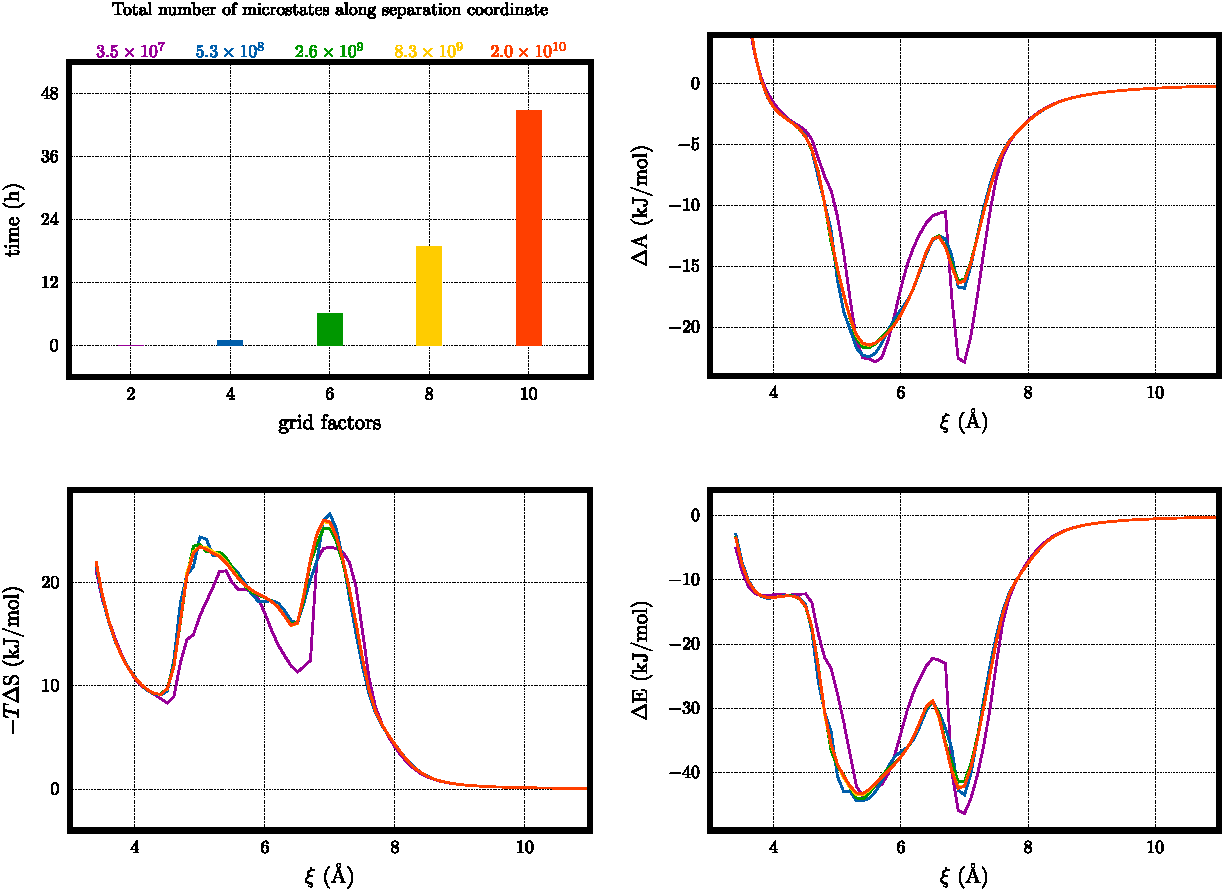
\includegraphics[width=1.0\textwidth]{figures/benchmark_cys.pdf}
  \caption{Comparison of calculation wall-time (in hours) and thermodynamic
           properties as a function of the grid coarseness for the association 
           of (L)-CYS dimers.}
  \label{fig:benchmark}
\end{figure}

  As one can notice, the cheapest calculation (grid factor = 2, purple curves) resulted in thermodynamic 
profiles considerably different, due to poorly sampling phase space regions with higher
entropic loss. For grid factor = 4 (blue curves), although results are improved,
one can still observe noticeable differences in comparison to the more costly
calculations. On the other hand, for grid factor >= 6, only small differences
are observed, indicating a good convergence for all thermodynamic profiles.

\bibliography{references}

\end{document}


